\chapter{توابع و ساختارها}

\section{ \textbf{ساختارها}}

\subsection{\lr{sph-skein-big-context}}
\label{subsec:sph-skein-big-context}
این ساختار مورد نظر برای ذخیره و استفاده از هش است (‌ شامل مقادیری از هش قبلی و مقادیر جدید محاسبه شده ). \\ این ساختار شامل یک آرایه‌ی ۶۴ بیتی از کاراکترهاست که به منظور تراز کردن انواع هش استفاده می‌گردد و  هشت عدد ۶۴ بیتی  که برای ذخیره‌ی ۵۱۲ بیت هش  استفاده می‌شوند  و هم‌چنین شامل دو عدد با نام‌های \lr{ptr, bcount} است که این دو عدد به طور معمول برابر ۰ هستند که همانند \lr{nonce} در پیاده‌سازی وریلاگ آن است.



\subsection{\lr{IV512}}
\label{subsec:IV512}
این ساختار شامل مقادیر اولیه‌ی هش است. یک عدد ۵۱۲ بیتی را برای خوانا بودن در مبنای ۱۶ و در ۸ بلاک ۱۶ بیتی نگاه می‌دارد. این مقدار در برنامه‌ به زبان وریلاگ همان \lr{midstate} است.
\subsection{\lr{UBI-BIG}}
\label{subsec:UBI-BIG}
این تابع  (  در مدل‌طلایی به صورت \lr{define} تعریف شده )  طبق الگوریتم \lr{skein} در ابتدا وظیفه‌ی ۵۱۲ بیتی کردن ورودی در بافر را بر عهده دارد، در ادامه تمامی ۷۲ مرحله‌ی هش الگوریتم \lr{skein} را که در مقدمه شرح داده شده است را اجرا می‌کند.
\\
روند اجرای این تابع بدین صورت است که در ابتدا مقادیر ۸ بیتی در بافر را با استفاده از \lr{Encoder} به مقادیر ۶۴ بیتی تبدیل می‌کند، سپس دو مقدار $t_0 , t_1$
را که همان $ tweak $ ها هستند را با استفاده از ورودی‌ها به‌دست می‌آورد و سپس با استفاده از تابع \hyperref[subsec:TFBIG-INIT]{\lr{TFBIG-INIT}} مقادیر جدیدی از داده‌های قبلی به دست می‌آورد،‌ سپس ۱۸ بار توابع \hyperref[subsec:TFBIG-4e]{\lr{TFBIG-4e}} و \hyperref[subsec:TFBIG-4o]{\lr{TFBIG-4o}} صدا می‌شوند که در هر کدام از‌ این تابع‌ها ۴ بار تابع درهم‌سازی توضیح داده شده در مقدمه صدا می‌شوند.


\subsection{\lr{TFBIG-4e}و \lr{TFBIG-4o}}
\label{subsec:TFBIG-4e}
\label{subsec:TFBIG-4o}

این تابع برای کدگذاری $ P_0 $ تا $ P_7 $ طراحی شده‌است. همان‌طور که پیش‌تر توضیح داده شده است، ۷۲ بار تابع درهم‌سازی صدا می‌شود،‌ و هر ۸ سلسله از این ۷۲ مرحله یکسان است، هم‌چنین در هر ۸ سری ۴ بار با یک کلید و ۴ بار دیگر با یک کلید دیگر اجرا می‌شود،‌ که به همین دلیل این توابع  هر کدام برای آن ۴ باری استفاده می‌شود که در مرحله‌ای زوج یا فرد قرار داریم.
\\
این تابع یک ورودی  \lr{s} دارد. تابع  \hyperref[subsec:TFBIG-ADDKEY]{\lr{TFBIG-ADDKEY }} با ‌$ p_0 $ تا  $ p_7 $ و $ h $ و $ t $و ‌$ s $ به ترتیب به عنوان  $ w_0 $ تا $ w_7 $و $ k $و ‌$ t $ و ‌$ s $ صدا شده‌است. ‌$ h $ و $ t $ برای \lr{concat} و ساختن کلید در تابع \lr{TFBIG-ADDKEY} استفاده شده‌اند.
سپس   \hyperref[subsec:TFBIG-MIX8]{\lr{TFBIG-MIX8 }}چهار بار برای ترتیب‌های متفاوتی از ‌$ p_0 $ تا $ p_7 $ اعداد متفاوت به عنوان $ rc $ صدا شده‌است. ترتیب صدا شدن $ p_0 $ تا $ p_7 $ برای تعداد بلاک ۸ به صورت جدول‌های زیر است،‌ که برای هر ‌‌راند از ۰ تا ۳، بر حسب راند قبل ترتیب‌ها چهار عدد جابه‌جا شده‌اند. و تفاوت حالت‌های زوج و فرد در اعداد استفاده شده است.
\begin{center}
	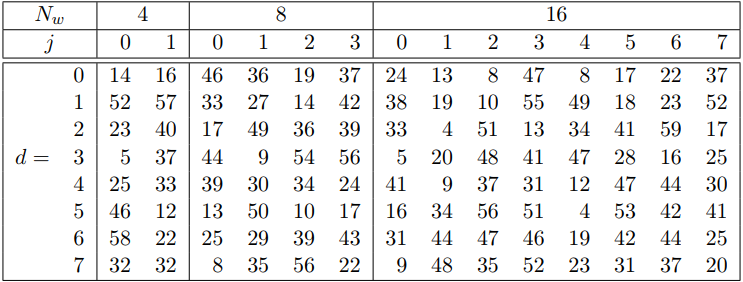
\includegraphics[width=10cm]{images/table_mix.png}
	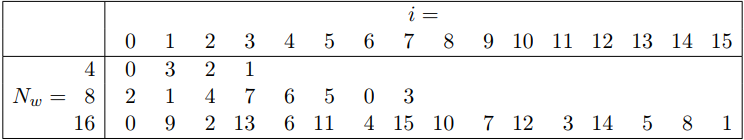
\includegraphics[width= 10cm]{images/Mix2.png}
\end{center}


\subsection{\lr{TFBIG-ADDKEY}}
\label{subsec:TFBIG-ADDKEY}

این تابع طبق فرمول‌های زیر مقادیر ورودی را تغییر می‌دهد و برای اینکار از تابع‌های \hyperref[subsec:SKBI]{\lr{SKBI}} و \hyperref[subsec:SKBI]{\lr{SKBT}} استفاده می‌کند که به ترتیب جمع مقادیر ورودی‌شان را به پیمانه ۳ و ۹ محاسبه می‌کنند.

\begin{latin}
	\begin{center}
		\begin{tabular}{c c}
			$k_{s, i} = k_{(s+i) \mod 9} $ \hspace{15mm} & $  i = 0, 1, 2, ... , 4 $ \\
			
			
		\end{tabular}
	\\
	$k_{s, 5} = k_{(s+5) \mod 9} + t_{s \mod 3}$ \\
	$k_{s, 6} = k_{(s+6) \mod 9} + t_{(s+1) \mod 3}$ \\
	$k_{s, 7} = k_{(s+7) \mod 9} + s $\\
	
	\end{center}

\end{latin}


دقت شود که تمامی این محاسبات برای نوع ۵۱۲ بیتی الگوریتم است.



\subsection{\lr{SKBT} و \lr{SKBI}}
\label{subsec:SKBI}

تابع \lr{SKBI} برای محاسبه‌ی اندیس کلید استفاده‌ شده‌است. \\ 
در الگوریتم برای تولید $k_0 $ تا $ k_8 $ از این ماکرو استفاده شده ‌است.  ,این ماکرو $ k $ و $ s $ و $ i $ را گرفته و سپس $ k $ را به \lr{ M9-s-i }متصل می‌کند که باقی‌مانده‌ی ‌$s + i $بر ۹ تعریف شده‌است.
تابع \lr{SKBT} مشابه تابع بالاست با این تفاوت که در انتها باقی‌مانده عدد را بر ۳ محاسبه می‌کند و از این تابع برای به‌دست آوردن اندیس \lr{tweak} ها استفاده می‌شود.


\subsection{\lr{TFBIG-MIX8}}
\label{subsec:TFBIG-MIX8}


همان‌طور که در مقدمه گفته‌ شده‌است،‌ هر سری از هشت سری، چهار \lr{round} دارد، پس طراحی این تابع برای ساده‌سازی استفاده‌ی متداول از \hyperref[subsec:TFBIG-MIX]{\lr{TFBIG-MIX}} بوده‌است. به صورت متداول در کد به چهار سری استفاده از  \lr{TFBIG-MIX}پشت سر هم نیاز است. 


\subsection{\lr{TFBIG-MIX}}
\label{subsec:TFBIG-MIX}

وظیفه‌ی این تابع درهم سازی بلاک‌های ورودی طبق فرمول‌های زیر است.
\begin{center}
	$y_0 = (x_0 + x_1) \mod 2^{64}$ \\
	$ y_1 = (x_1 <<< R_{(d \mod 8), j}) \oplus y_0$
\end{center}
\\
که مقادیر $ R $ در جدول زیر آمده است :

\begin{center}
	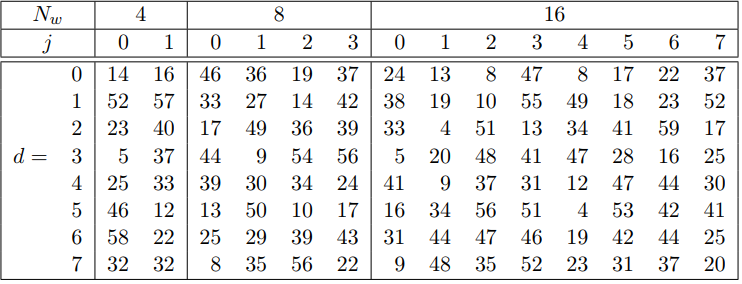
\includegraphics[width=10cm]{images/MIX1.png}
\end{center}




\subsection{\lr{TFBIG-INIT}}
\label{subsec:TFBIG-INIT}
این تابع با ورودی‌های $ t_0 $ تا $ t_2 $ و $h_0 $ تا $ h_8 $ مقادیر زیر را محاسبه می‌کند :
$$
k_8 = C \oplus k_0 \oplus k_1 \oplus ... \oplus k_7
$$

$$
	t_2 = t_1 \oplus t_0
$$
 که مقدار ثابت $ C $ به آن جهت در فرمول وجود دارد که از ۰ نبودن تمامی بیت‌ها اطمینان حاصل شود.
\section{ توابع}

\subsection{\lr{sph-skein512-init}}
\label{subsec:sph-skein512-init}
این تابع مسئولیت مقداردهی اولیه‌ی ساختار هش را بر عهده دارد، که برای آن تابع \hyperref[subsec:skein-big-init]{\lr{skein-big-init}} را با ورودی‌ اولیه‌ی \lr{IV512} اجرا می‌کند.
\subsection{\lr{skein-big-init}}
\label{subsec:skein-big-init}

این تابع دو ورودی می‌پذیرد که یکی از آن‌ها آدرس یک ساختار هش است و دیگری مقدار اولیه، که مقادیر متناظر ساختار داده شده را برابر مقادیر اولیه قرار می‌دهد.
که مقدار اولیه در حالت ۵۱۲ بیتی در ساختار \lr{IV512} ذخیره شده ‌است.

\subsection{\lr{sph-skein512}}
\label{subsec:sph-skein512}
این تابع، مقدار هش محاسبه شده تا این لحظه را از بین می‌برد و 